\section{Initialization}
The number of particles $N$ is given by $4M^3$, where $M$ is the number of unit cells per dimension. The particles are then placed in the unit cell using a fcc Bravais lattice structure, with lattice constant $a=L/M$. Using the density $\rho$ and $N$, the size of the volume $V$ is determined and filled with the unit cells. Overlapping particles are avoided, by filling each unit cell with only the lower left 4 particles, as shown in figure \ref{fig:unit_cell}. The unit cells near the boundaries are given an offset of $a/10$, to avoid ambiguity of these particle locations.
\begin{Figure}
 \centering
 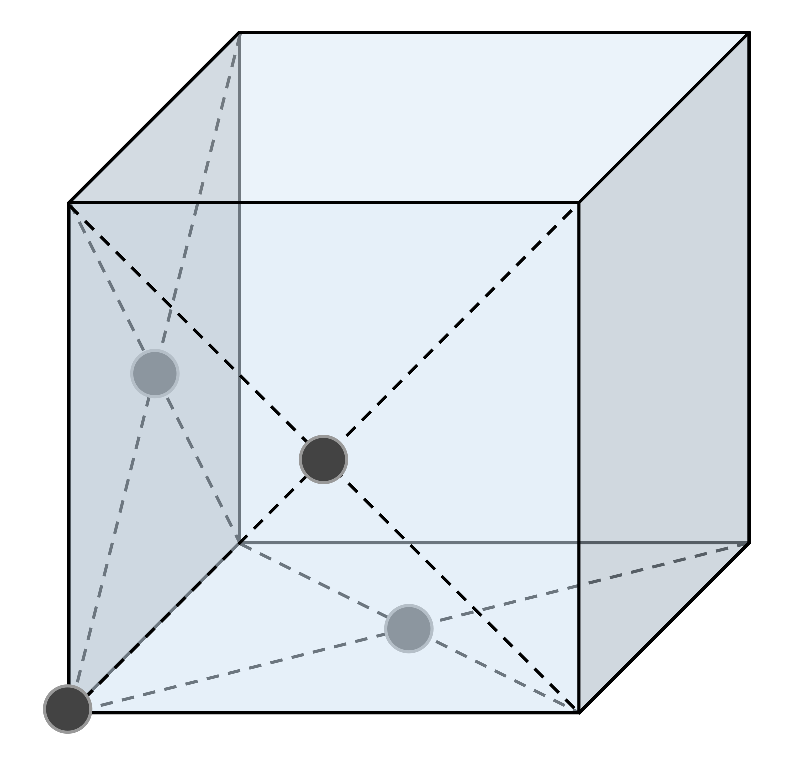
\includegraphics[width=0.35\linewidth]{fcc_cell.eps}
 \captionof{figure}{fcc Bravais unit cell.}\label{fig:unit_cell}
\end{Figure}

The particles are given an initial velocity with Maxwell distribution, $ $. The distribution can be rewritten to: [[see JMT for full derivation]]

[[reduced units]]

Lennard-Jones pair potential:
\begin{gather*} 
    U(r) = 4\epsilon\left[\left(\frac{\sigma}{r}\right)^{12}-\left(\frac{\sigma}{r}\right)^6\right].
\end{gather*}

The initialization functions are combined in the 